\chapter{Základní pojmy}

\section{Šum}

V teorii detekce signálu šumem nazýváme jakoukoli nechtěnou (a typicky neznámou) modifikaci signálu.

\subsection{Barva šumu}

U aditivního šumu můžeme měřit intenzitu šumu na různých frekvencích. Šumu se
říká bílý šum, pokud by světlo, které by mělo stejnou distribuci intenzity
napříč frekvencemi, jako daný šum (který ale vůbec nemusí být světelný), bylo
bílé. Podobně známe například ještě růžový, hnědý či modrý šum.

Intenzita $p$ všech zmíněných šumů na v na dané frekvenci lze vyjádřit jako
$p=1/f^\beta$, kde hodnota $\beta$ je $-1$ pro modrý šum, $0$ pro bílý, $1$ pro
růžový a $2$ pro hnědý. Proto se růžový šum někdy též označuje jako $1/f$ šum. Pro
ostatní barvy šumu není podobné označení běžné. 

V této práci se budeme zabývat vizuálním šumem, tedy šumem, kde místo obvykle
používané časové souřadnice použijeme dvě souřadnice prostorové, a měřenou
hodnotou bude jas. 

\begin{figure}[h!]
\begin{tabular}{cc}
\begin{subfigure}{0.45\textwidth}
  \centering
  
\includegraphics[width=.8\linewidth]{img/blue_noise}
  \caption{Modrý šum} 
\end{subfigure}&
\begin{subfigure}{0.45\textwidth}
  \centering
  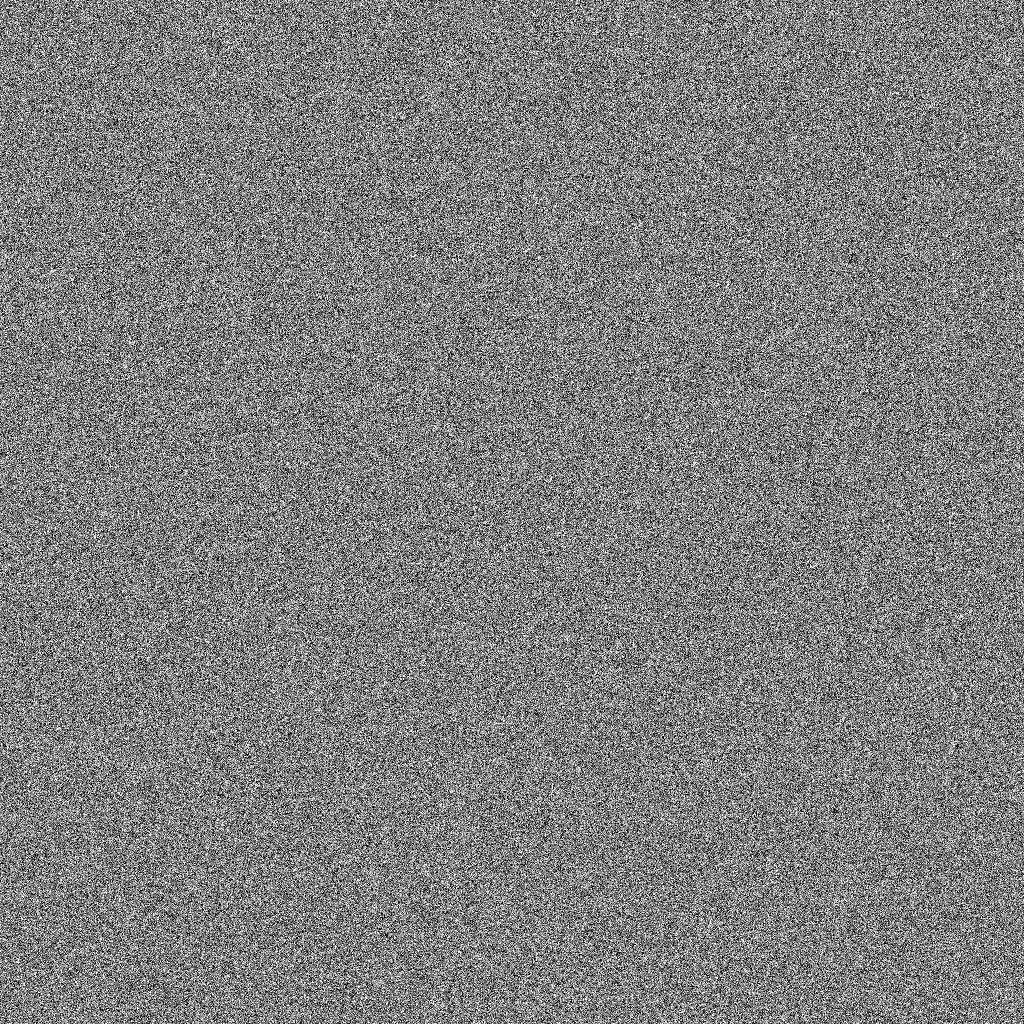
\includegraphics[width=.8\linewidth]{img/white_noise}
  \caption{Bílý šum} 
\end{subfigure}\\
\begin{subfigure}{0.45\textwidth}
  \centering
  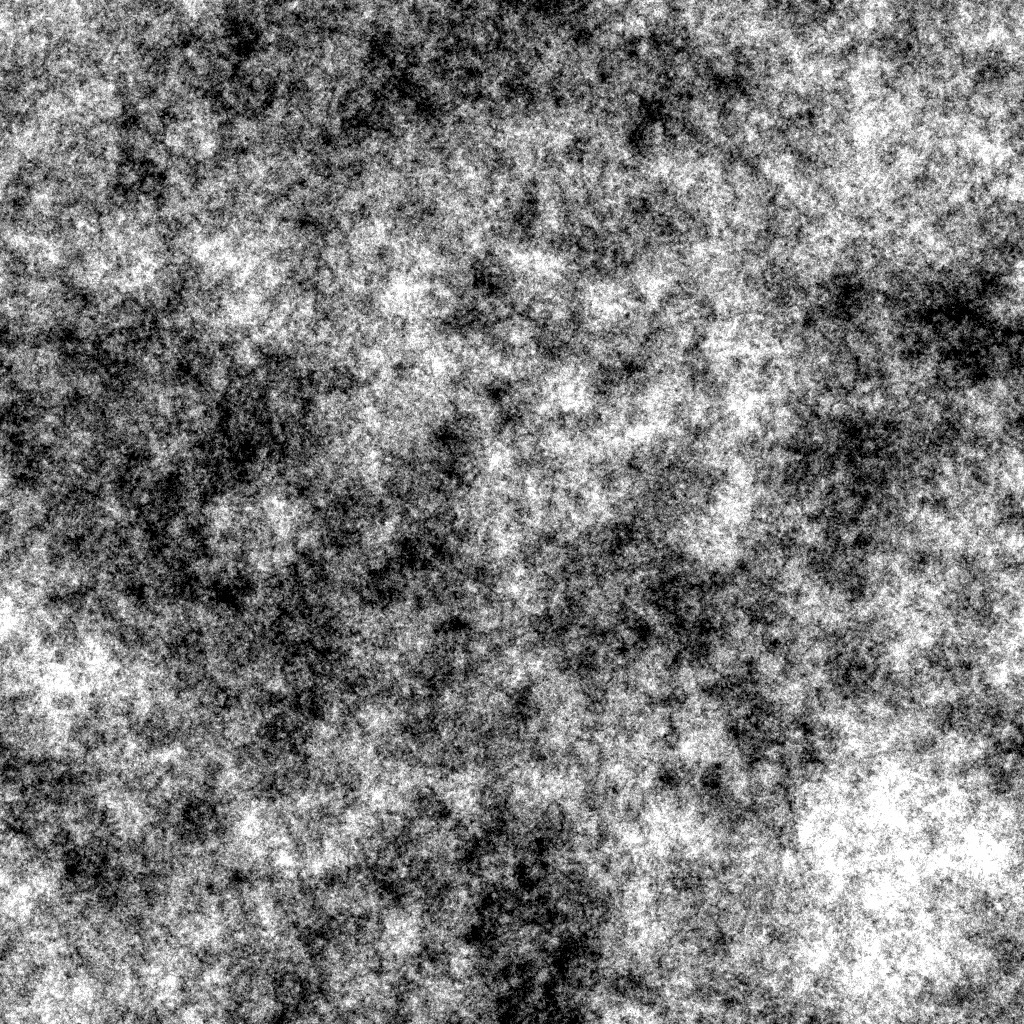
\includegraphics[width=.8\linewidth]{img/pink_noise}
  \caption{Růžový šum} 
\end{subfigure}&
\begin{subfigure}{0.45\textwidth}
  \centering
  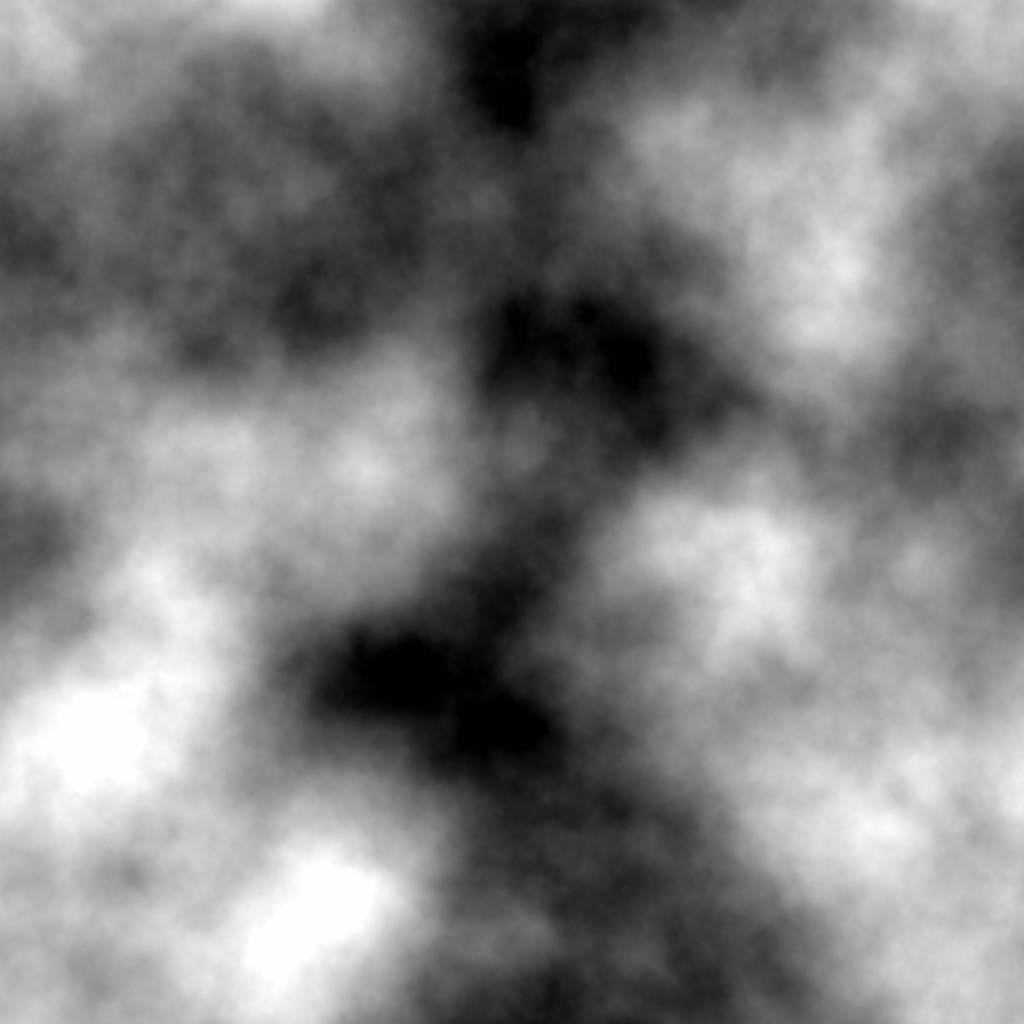
\includegraphics[width=.8\linewidth]{img/brown_noise}
  \caption{Hnědý, někdy též červený nebo Brownův šum} 
\end{subfigure}%
\end{tabular} 
\caption{Ukázky různých šumů.} 
\label{obr:noise:example} 
 
\end{figure}
\section{Gabor patch}

Gabor filter (v českých textech někdy označovaný jako Gaborova vlnka) je
lineární filtr používaný ve zpracování obrazu, chceme-li detekovat signál
mající danou frekvenci a směr, který se vyskytuje kolem daného bodu.

\subsection{Definice}

Hodnotu filtru v daném bodě spočítáme jako součin dvou funkcí. První z nich je
vždy sinus či cosinus (někdy uváděné v podobě komplexní exponenciály, pokud
potřebujeme i reálnou, i imaginární složku). Jeho parametry určují, jaké
vlastnosti má mít signál, který chceme detekovat. Druhé funkci říkáme obálka, a
určuje, na jakém okolí daného bodu signál zkoumáme.

Funkce tedy vypadá jako $$g(x,y) =
\sin\left(2\pi\frac{x'}{\lambda}+\phi\right)*\operatorname{obálka}(x',y'),$$
kde vektor $(x',y')^T$ je vektor $(x,y)^T$ otočený o úhel, který svírá osa $x$
se směrem, podél nějž chceme měřit signál (tento úhel budeme značit $\Theta$),
a posunutý do bodu, v němž chceme měřit signál, $\lambda$ je frekvence signálu,
který hledáme, a $\phi$ je fázový posun.

Jako obálka se používá dvojrozměrná Gaussova funkce, raised cosine, nebo prostá lineární funkce vzdálenosti. 

Gaussovu funkci vyjádříme jako $$ \operatorname{obálka}(x,y) =  \exp\left(\frac{x'^2 +
y'^2}{2\rho}\right),$$ kde $\rho$ je směrodatná odchylka Gaussovy křivky. Její výhodou je, že chování Gabor filtru, jehož obálku tvoří Gaussova funkce, je nejlépe popsané. Raised cosine vyjádříme jako 
$$
\operatorname{obálka}(x,y)=
\begin{cases}
 \frac{\cos(\pi\sqrt{x'^2+y'^2}/r)+1}2 &\text{pro $\sqrt{x'^2+y'^2}\leq r$,}\\[1ex]
 0 &\text{jinak,}
\end{cases}
$$ kde $r$ je poloměr oblasti, v níž chceme signál detekovat. Výhodou raised cosine oproti Gaussově funkci je, že ve vzdálenosti alespoň $r$ od středu filtru jeho hodnota nabývá nuly. Při výpočtech tedy stačí počítat s malou oblastí kolem středu (kdežto při použití Gaussovy funkce je nutné počítat s celým obrazem). Výhodou oproti lineární funkci vzdálenosti je, že raised cosine se pro většinu aplikací chová dostatečně podobně, jako Gaussova funkce.

\subsection{Použití}

Chceme-li detekovat signál ve vizuálním šumu, spočítáme hodnotu $$s=\sum g(x,y)*n[x,y],$$ kde $n$ je šum a sumu bereme přes všechny body $(x,y)$, v nichž jsme naměřili hodnoty šumu. Je-li hodnota $s$  blízko nuly, signál v daném místě
není přítomen, nebo je přítomen s jinými parametry. Vysoké hodnoty značí, že
signál pravděpodobně přítomen je, hluboce záporné značí, že signál je přítomen,
ovšem s fází posunutou $\pi$.

Gabor filter ale můžeme používat i k samotné tvorbě signálu. Chceme-li vytvořit
v nějakém bodě signál, můžeme spočítat Gabor filter, jako bychom chtěli
detekovat signál s právě takovými parametry, jaké má mít tvořený signál, a potom ho sečíst se šumem. Takto vytvořenému signálu budeme říkat
Gabor patch.

\begin{figure}[h!]
\begin{subfigure}{0.25\textwidth}
  \centering
  
\includegraphics[width=.8\linewidth]{img/gabor1}
\end{subfigure}% 
\begin{subfigure}{0.25\textwidth}
  \centering
  
\includegraphics[width=.8\linewidth]{img/gabor2}
\end{subfigure}% 
\begin{subfigure}{0.25\textwidth}
  \centering
  
\includegraphics[width=.8\linewidth]{img/gabor3}
\end{subfigure}% 
\begin{subfigure}{0.25\textwidth}
  \centering
  
\includegraphics[width=.8\linewidth]{img/gabor4}
\end{subfigure}% 
\caption{Ukázky několika Gabor patchů. Všechny gabor patche jsou 100 pixelů široké i vysoké. Levý patch má $\Theta = 1/4\pi$, ostatní mají $\Theta = -1/4\pi$, levý má jako obálku Gaussovu funkci, prostřední dva raised cosine, pravý lineární funkci vzdálenosti, první, druhý a čtvrtý mají frekvenci (v cyklech na pixel) $0.1$, třetí $0.02$.} 
\label{obr:gabor:example} 
 
\end{figure}


\section{Ideální bayesovský pozorovatel}
